\documentclass[polish,polish,a4paper]{article}
\usepackage[utf8]{inputenc}
\usepackage{polski}


\usepackage[letterpaper,top=2cm,bottom=2cm,left=3cm,right=3cm,marginparwidth=1.75cm]{geometry}

% Useful packages
\usepackage{amsmath}
\usepackage{graphicx}
\usepackage{hyperref}

    
\title{Mobilny robot klasy minisumo "Stefan" }
\author{Kamil Winnicki}

\begin{document}
\begin{titlepage} %crea l'enviroment
\begin{figure}[t] %inserisce le figure
    \centering
\includegraphics[width=0.6\textwidth]{zdjecia/sprite_src_konar_vertical.jpg}
\end{figure}
\vspace{20mm}

\begin{Large}
 \begin{center}
	\textbf{Koło naukowe robotyków KoNaR\\ Politechnika Wrocławska\\}
	\vspace{30mm}
    

        
            \hrule
            \vspace{10mm}
	{\huge{\bf Projekt robota mobilnego klasy minisumo "Stefan"}}
            \vspace{10mm}
            \hrule
\end{center}
\end{Large}


\vspace{36mm}
%minipage divide la pagina in due sezioni settabili
\begin{minipage}[t]{0.47\textwidth}
	
\end{minipage}
\hfill
\begin{minipage}[t]{0.47\textwidth}\raggedleft
	{\large{\bf Autor:\\ Kamil Winnicki}}
\end{minipage}

\vspace{25mm}

\hrulefill

\vspace{5mm}

\centering{\large{\bf Luty 2023 }}

\end{titlepage}




\tableofcontents
\newpage
\begin{figure}[!htb]
       \begin{minipage}{0.3\textwidth}
         \centering
         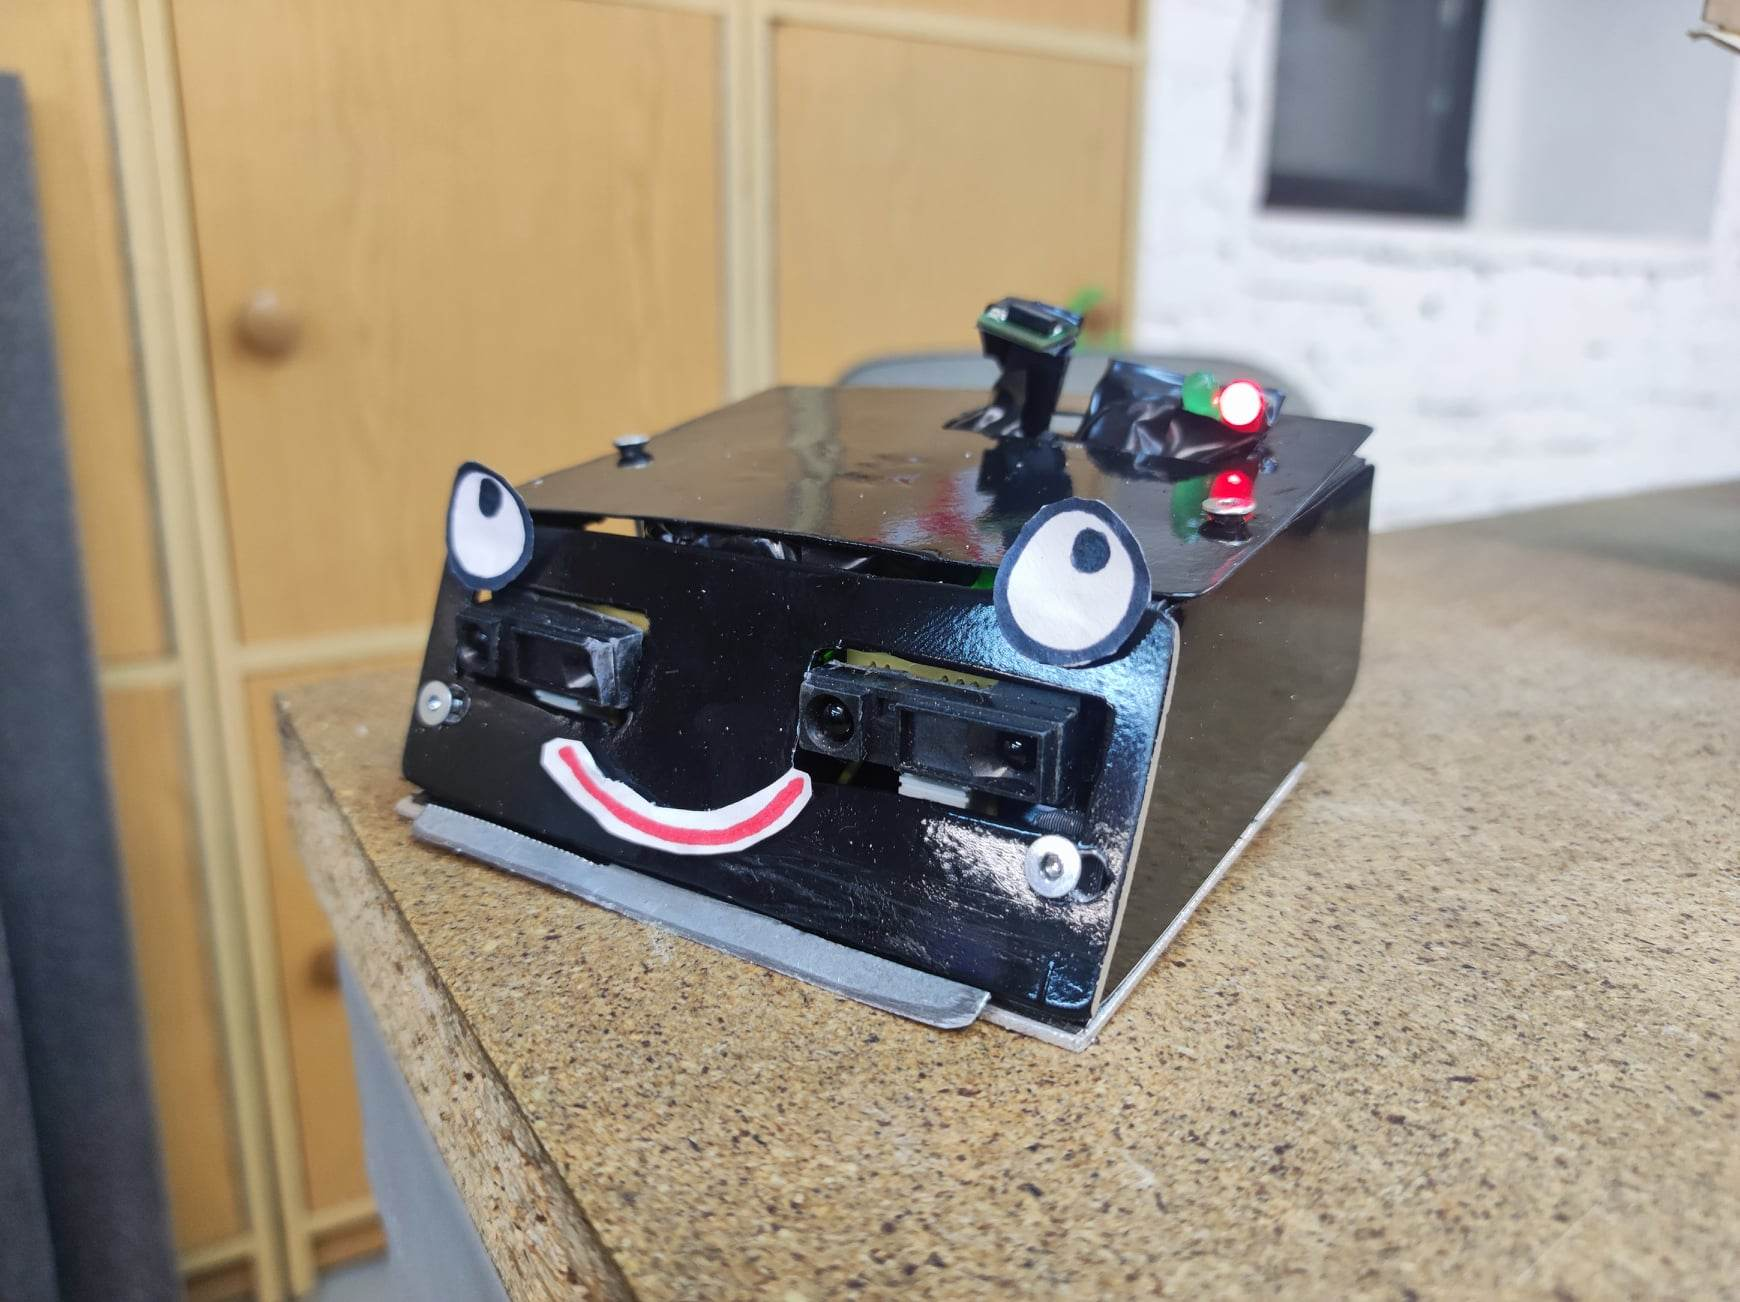
\includegraphics[width=1.5\linewidth]{zdjecia/Stefanwpiwnicy.jpg}

       \end{minipage}\hspace{34mm}
       \begin{minipage}{0.3\textwidth}
         \centering
         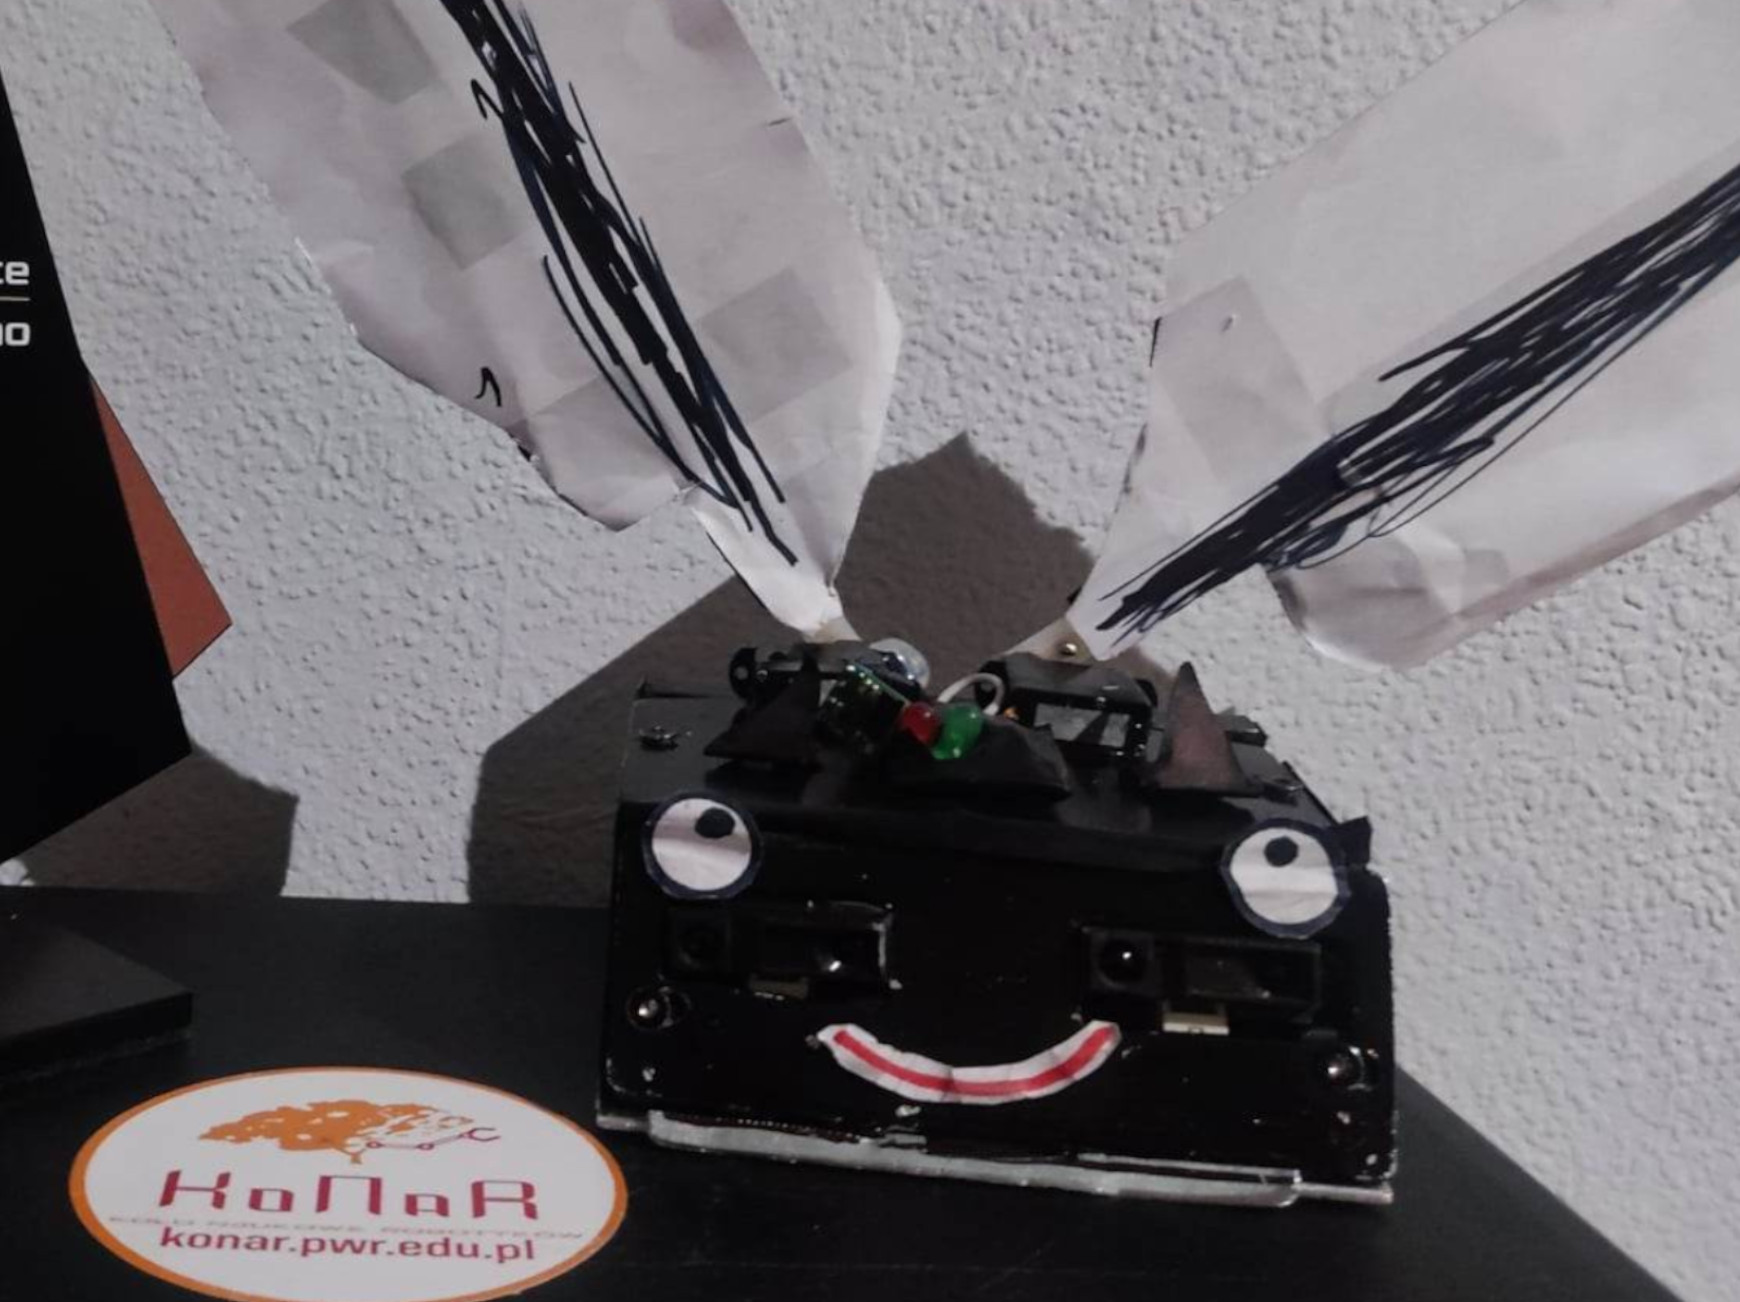
\includegraphics[width=1.5\linewidth]{zdjecia/Stefek.jpg}

       \end{minipage}
        \end{figure}

\section{Wstęp}

Pierwszy pomysł na powstanie robota powstał po zawodach robotycznych w Rybniku w 2022 roku. Stworzenie robota było możliwe dzięki dużej pomocy kolegów z koła naukowego robotyków "KoNaR".

\section{Kategoria turniejowa Minisumo}

Zawody robotów w kategorii sumo wzorowane są na japońskich zapasach sumo. Przeciwnikami są dwa autonomiczne roboty, które próbują wypchnąć rywala poza powierzchnię ograniczonego białą linią czarnego koła ringu (tzw. dohyo). Zazwyczaj walki robotów sumo składają się z 3 kilkuminutowych rund a zwycięzcą jest robot, który dwukrotnie wypchnie przeciwnika poza ring. Zawodnicy nie mają kontroli nad robotami. Jedyną rzeczą jaką mogą wykonać  jest uruchomienie pilotem procedury startowej. W czasie zmagań robot musi działać już autonomicznie.  

\section{Założenia projektowe}
\begin{itemize}
  \item Spełnienie fizycznych ograniczeń regulaminu kategorii minisumo (rozmiar max 100x100 mm oraz maksymalna waga 500g)
  \item W pełni autonomiczne działanie robota (poruszanie się, wykrywanie i wypchanie przeciwnika, kontrola krawędzi ringu) 
  \item Sterowanie oparte o mikrokontroler firmy Atmel, Atmega328p-au na płytce Arduino nano
  \item Dwa silniki sterowane różnicowo
  \item Dwa czujniki wykrywające przeciwnika
  \item Dwa czujniki wykrycia linii

\end{itemize}



 


\newpage

\section{Elektronika}
    Elektronika została wykonana na płytce uniwersalnej, jednostronnej. 
    \subsection{Płytka Arduino nano}
        Wybór płytki Arduino nano jako głównego sterowania został dokonany ze względu na uproszczenie wykonania elektroniki oraz znajomość środowiska Arduino.
       
        \begin{figure}[!htb]
       \begin{minipage}{0.3\textwidth}
         \centering
         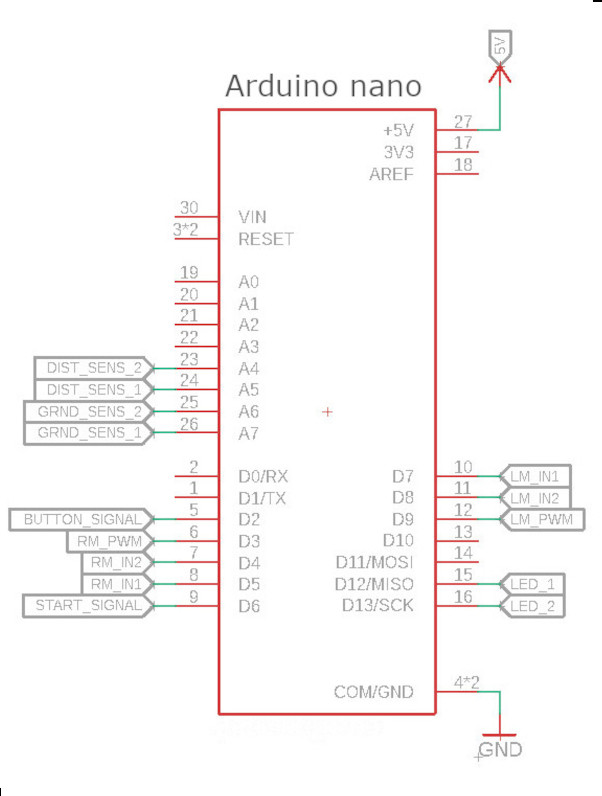
\includegraphics[width=2.3\linewidth]{Scheme/Arduino.jpg}
         \caption{Schemat podłączeń do płytki}\label{Fig:Data1}
       \end{minipage}\hfill
       \begin{minipage}{0.3\textwidth}
         \centering
         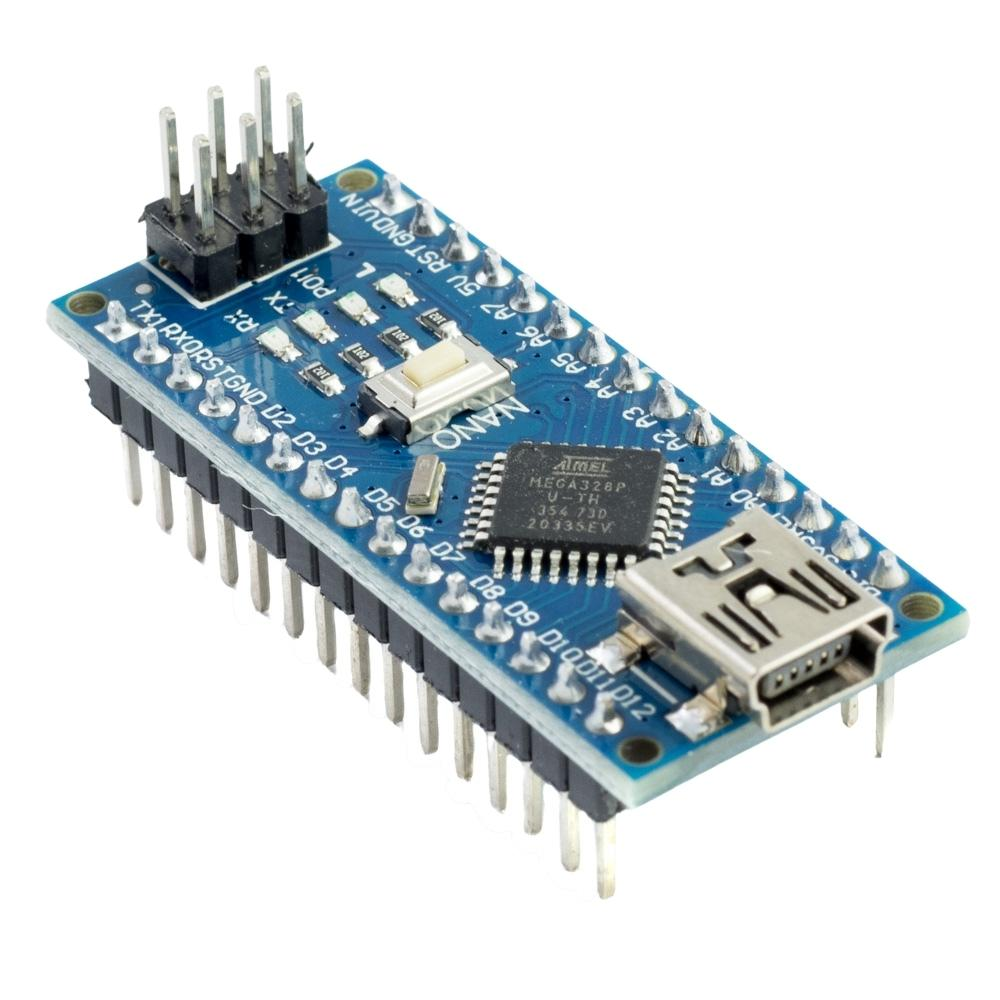
\includegraphics[width=1\linewidth]{photo/arduino.jpg}
         \caption{Płytka Arduino nano}\label{Fig:Data2}
       \end{minipage}
        \end{figure}
       
\newpage
    \subsection{Zasilanie}  

     \begin{figure}[!htb]
       \begin{minipage}{0.3\textwidth}

        \centering
        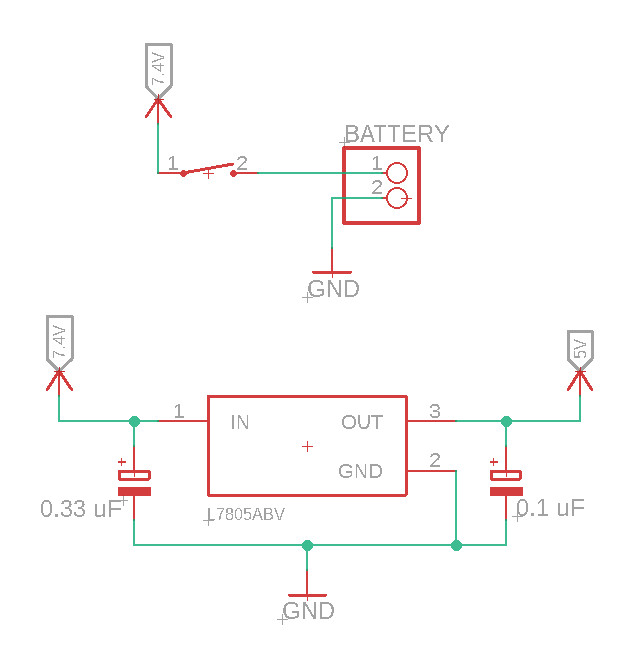
\includegraphics[width=75mm]{Scheme/zasilanie.jpg}
        
       \end{minipage} \hspace{35mm}
       \begin{minipage}{0.5\textwidth}
         
          Zasilanie zostało oparte o akumulator litowo - polimerowy 2S 7.4V, o pojemności 800mAh.  
        \newline
        \newline
        Ponieważ mikrokontroler atmega328p-au wymaga zasilania między 2.8V a 5V konieczne jest obniżenie napięcia. Został użyty do tego stabilizator liniowy LM7805. Płytka Arduino nano zawiera wbudowany stabilizator jednak został zastosowany zewnętrzny ze względu na jego niską wydajność prądową. W skrajnych przypadkach spowodowało by to przegrzanie stabilizatora, co z kolei mogłoby uszkodzić procesor.
        \newline
        \newline
        Dodatkowo w celu filtracji zasilania zostały zastosowane dwa kondensatory elektrolityczne.
        
       \end{minipage}
        \end{figure}

    \subsection{Silniki}
        Silniki wybrane do robota to N20-BT17 micro (zamienniki Pololu micro-series), o przekładni 50:1.
        \newline
        Jako sterownik silników użyty został TB6612FNG jako gotowy moduł.  
        
         \begin{figure}[ht!]
        \centering
        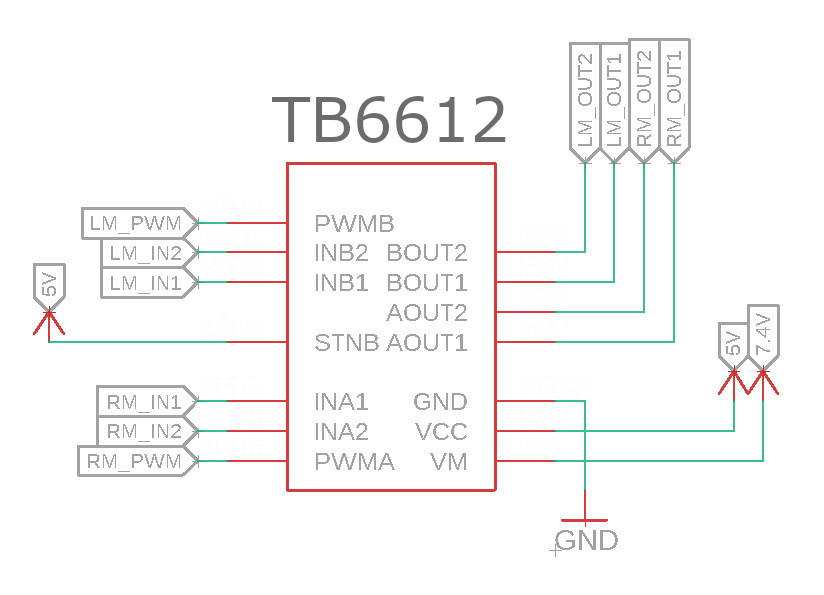
\includegraphics[width=80mm]{Scheme/Silniki.jpg}
        \caption{Schemat podłączenia sterownika\label{overflow}}
        \end{figure}   
        
        \begin{figure}[!htb]
       \begin{minipage}{0.3\textwidth}
         \centering
         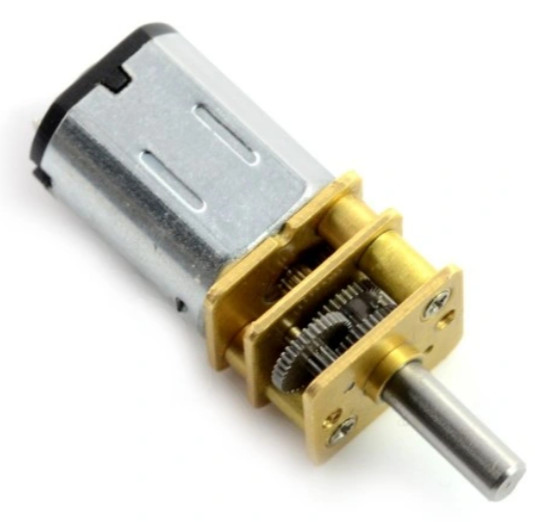
\includegraphics[width=.7\linewidth]{photo/silnik.jpg}
         \caption{Silnik}\label{Fig:Data1}
       \end{minipage}\hfill
       \begin{minipage}{0.3\textwidth}
         \centering
         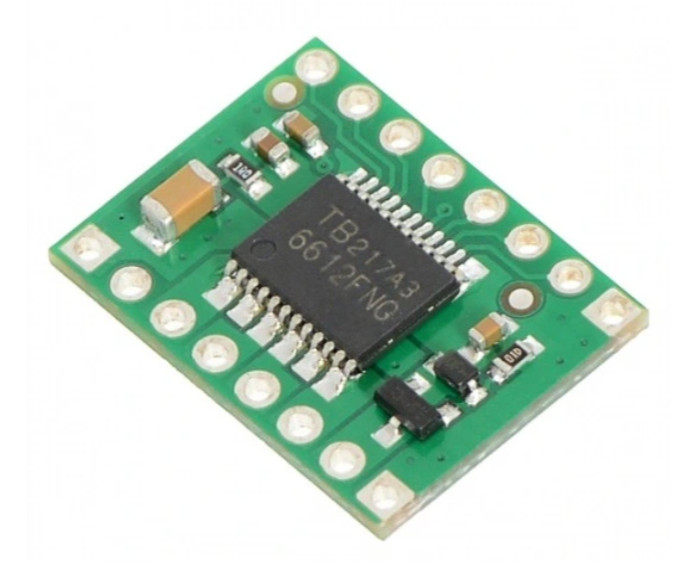
\includegraphics[width=.7\linewidth]{photo/TB6612FNG.jpg}
         \caption{Sterownik TB6612FNG}\label{Fig:Data2}
       \end{minipage}
        \end{figure}
    \newpage
    \subsection{Czujniki podłoża}
        Wykrywanie krawędzi ringu konieczne jest do unikniknięcia wypadnięcia robota z ringu. Do tego celu zastosowane zostały czujniki odbiciowe CNY70. Ich działanie opiera się o diode nadawczą oraz fotorezystor. Im światła odbitego jest więcej tym napięcie na wyjściu jest niższe. Krawędź ringu na zawodach pokryta jest białą farbą, kolor ten odbija światło bardziej niż czarne dlatego taki czujnik idealnie się do tego nadaje. W robocie zastosowano dwa takie czujniki, umieszczone z przodu.
        
        
        \begin{figure}[!htb]
       \begin{minipage}{0.3\textwidth}
         \centering
         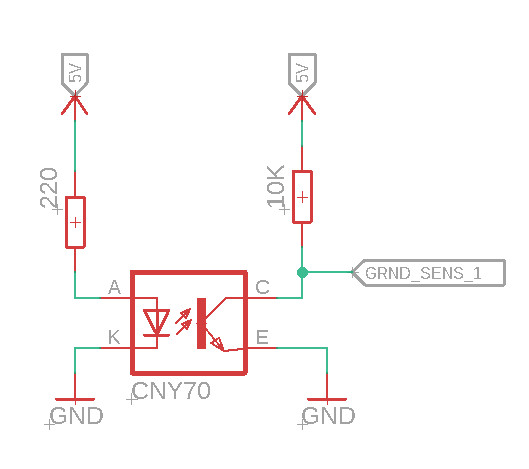
\includegraphics[width=1.8\linewidth]{Scheme/czujniki_ziemi.jpg}
         \caption{Schemat podłączenia czujnika}\label{Fig:Data1}
       \end{minipage}\hfill
       \begin{minipage}{0.3\textwidth}
         \centering
         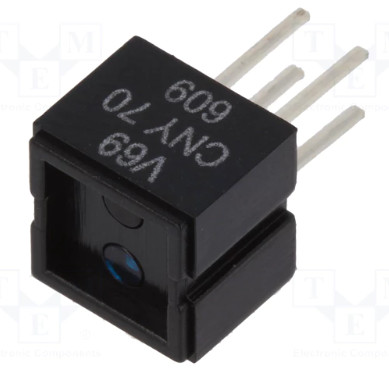
\includegraphics[width=.6\linewidth]{photo/Bez nazwy.jpg}
         \caption{CNY70}\label{Fig:Data2}
       \end{minipage}
        \end{figure}
        
    \subsection{Czujniki odległości}
        W celu wykrywania przeciwnika konieczne było zastosowanie czujników odległości. Wybór padł na analogowe czujniki optyczne SHARP GP2Y0A41SK0F, ponieważ w trakcie budowania robota miały one jeszcze przystępną cenę, są łatwe w obsłudze oraz szybkie w odczytach.
        
        \begin{figure}[!htb]
       \begin{minipage}{0.3\textwidth}
         \centering
         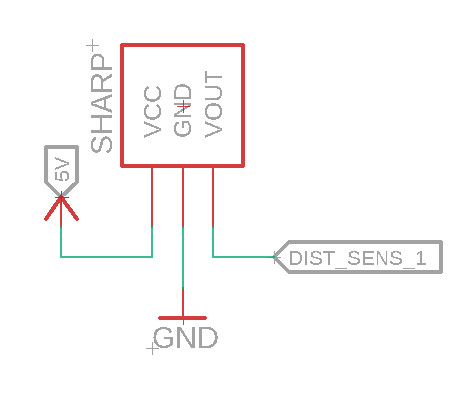
\includegraphics[width=1.7\linewidth]{Scheme/czujniki_odleglosci.jpg}
         \caption{Schemat podłączenia czujników}\label{Fig:Data1}
       \end{minipage}\hfill
       \begin{minipage}{0.3\textwidth}
         \centering
         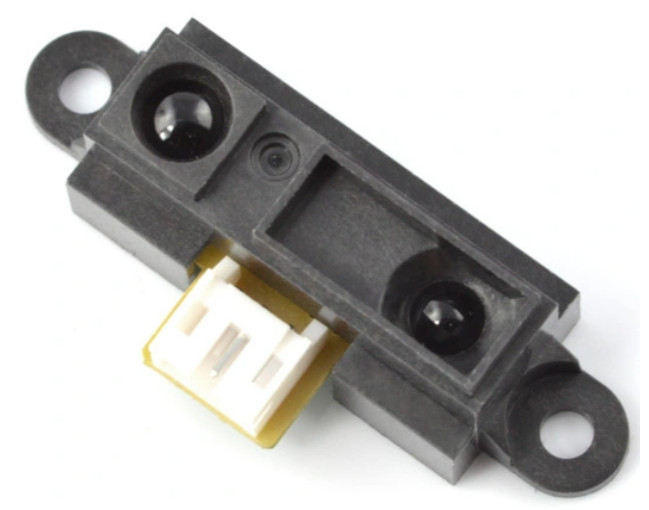
\includegraphics[width=.6\linewidth]{photo/sharp.jpg}
         \caption{Sharp GP2Y0A41SK0F}\label{Fig:Data2}
       \end{minipage}
        \end{figure}
\newpage
    \subsection{Interfejs użytkownika}
        "Interfejs użytkownika" zawiera dwie diody informujące o stanie w jakim znajduje się robot oraz przycisk do wyboru kierunku lub ręcznego startu. 
        
        \begin{figure}[ht!]
        \centering
        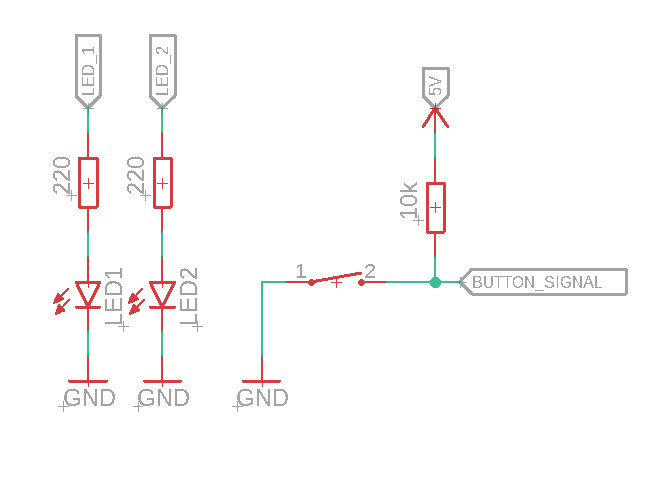
\includegraphics[width=90mm]{Scheme/interfejs.jpg}
        \caption{Schemat interfejsu \label{overflow}}
        \end{figure}
        
    \subsection{Starter}
    
    W celu zdalnego wystartowania robotów na zawodach stosuje się starter. Pozwala on na jednoczesne wystartowanie dwóch robotów w tym samym momencie co eliminuje zbyt wczesny start jednego z robotów. Na zawodach na całym świecie przyjęto ogólny standard starterów (wiedeński). Taki moduł startowy posiada odbiornik fali podczerwonej o częstotliwości 38kHz oraz diode informująca w jakim stanie znajduje się starter. Mrugnięcie dwa razy oznacza że starter został połączony z pilotem, brak świecenia czekanie na START, ciągłe świecenie oznacza START, ciągłe mruganie stan STOP. 
    \newline
    Moduł startowy zasilany może być napięciem od 3.3V do 5V. Posiada dwa piny sygnałowe: SIGNAL - podający stan wysoki w trakcie stanu START, oraz stan niski w trybie czekania i STOP. Kolejny pin to KILL, jednak jest on obowiązkowy tylko w kategorii MegaSumo, dlatego w tym robocie nie został podłączony.
    \newline 
    Wiecej informacji na temat startera można znaleźć na \href{https://p1r.se/startmodule/}{stronie} oraz \href{https://github.com/p1rse/robot-sumo-start-module}{GitHubie} twórcy.
    
    
    \begin{figure}[!htb]
       \begin{minipage}{0.3\textwidth}
         \centering
         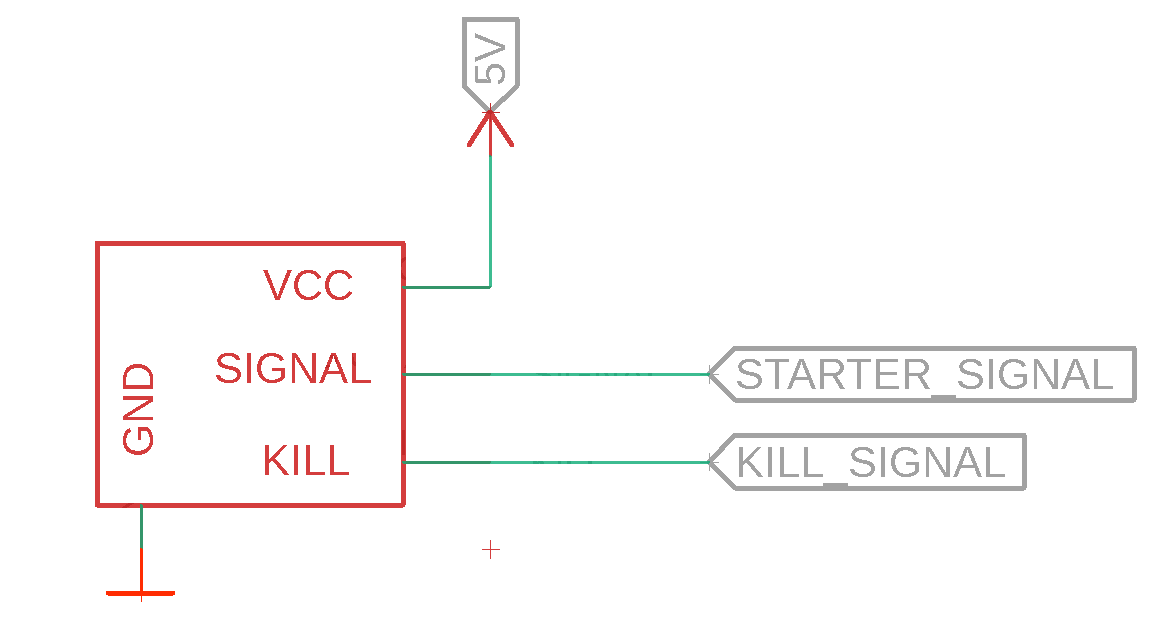
\includegraphics[width=1.7\linewidth]{Scheme/start.png}
         \caption{Schemat podłączenia startera}\label{Fig:Data1}
       \end{minipage}
       \hspace{40mm}
       \begin{minipage}{0.3\textwidth}
         
         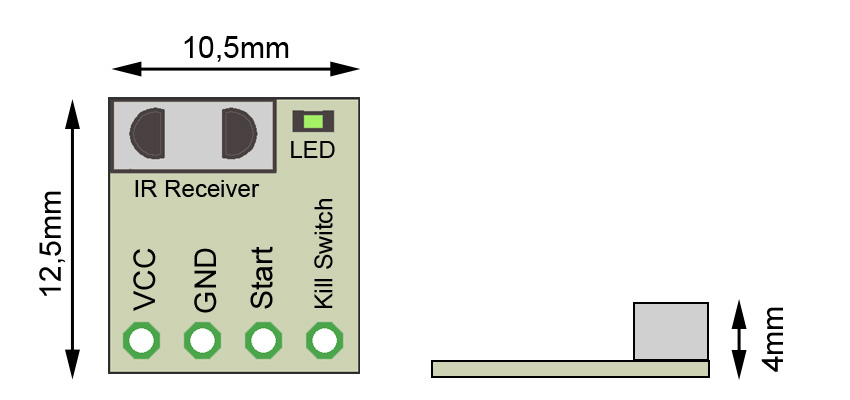
\includegraphics[width=1.6\linewidth]{photo/module-description_V0_03.jpg}
         \caption{Starter}\label{Fig:Data2}
         

       \end{minipage}
        \end{figure}
    \newpage
\section{Mechanika}
    Głównymi założeniami przy projektowaniu mechaniki było stworzenie robota możliwie jak najniższego oraz posiadającego obudowe z blachy. 
    
    
    \subsection{Rozmieszczenie elektroniki}
    Przy etapie tworzenia płytki z elektroniką należało uwzględnić odpowiednie rozmieszczenie elementów w taki sposób aby robot mógłby być możliwie jak najniższy. Niestety nie udało się tego osiągnąć w duzym stopniu przez baterię która okazała się zbyt duża. 
    
    \begin{figure}[ht!]
        \centering
        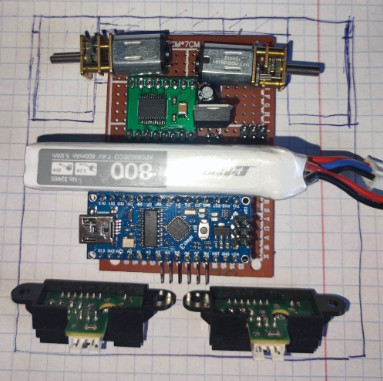
\includegraphics[width=50mm]{photo/srodek.jpg}
        \caption{Rozmieszczenie komponentów w srodku robota\label{overflow}}
        \end{figure}
    
    \subsection{Model 3D}
    W pierwszej kolejności projektowania mechaniki robota został stworzony pomocniczy model 3D który miał zapewnić łatwiejszą prace na dalszym etapie. 
    
        \begin{figure}[!htb]
       \begin{minipage}{0.3\textwidth}
         \centering
         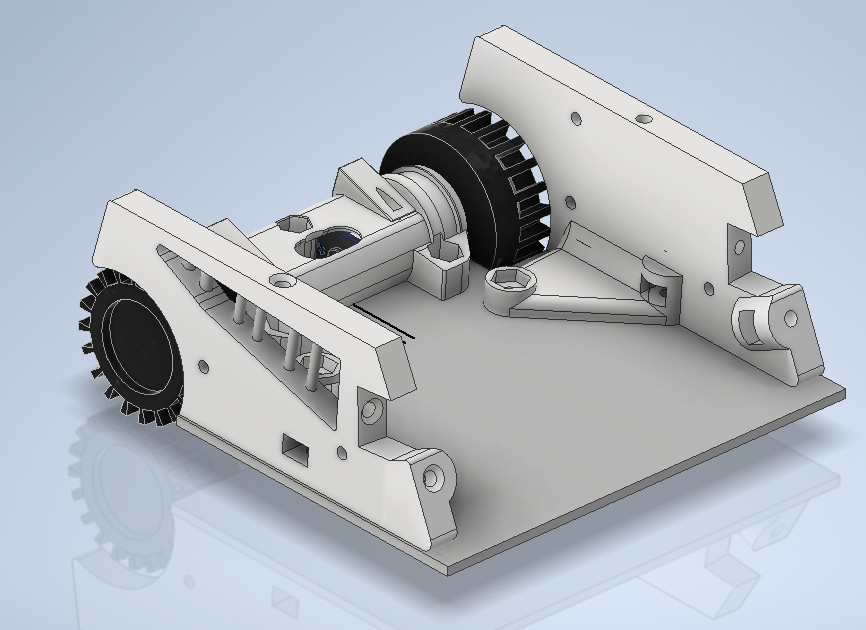
\includegraphics[width=1.55\linewidth]{photo/bez_pokryw.jpg}
         \caption{Model bez pokryw}\label{Fig:Data1}
       \end{minipage}\hspace{30mm}
       \begin{minipage}{0.3\textwidth}
         \centering
         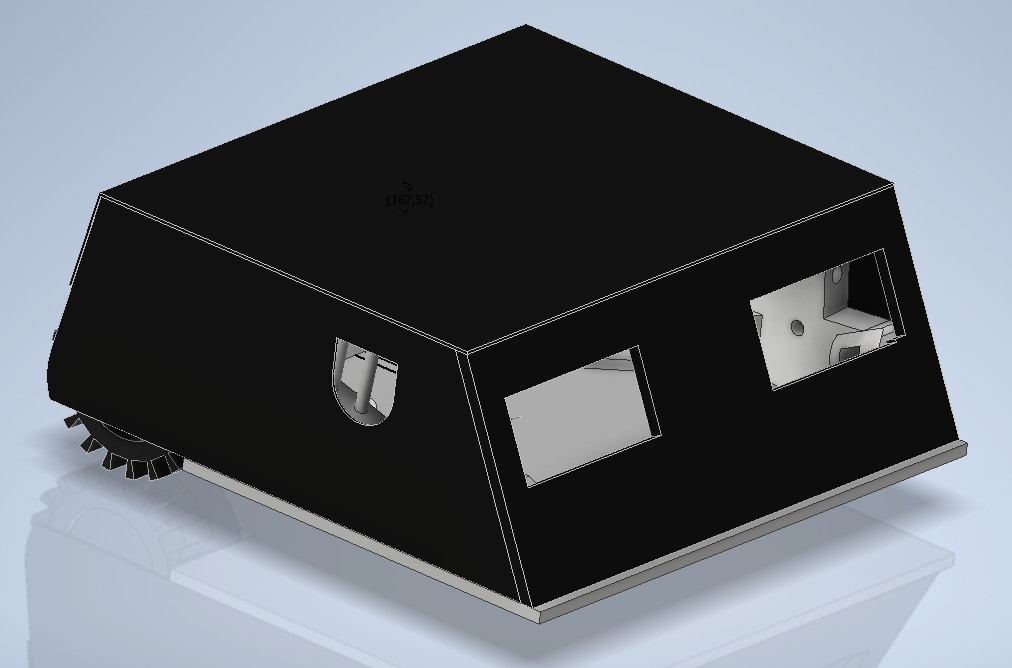
\includegraphics[width=1.69\linewidth]{photo/z_pokrywami.jpg}
         \caption{Model z pokrywami}\label{Fig:Data2}
       \end{minipage}
        \end{figure}
    
    
    \subsection{Konstrukcja}
        Do wykonania głównych ścianek mocujących oraz uchwytów na silniki użyto druku 3D. 
        Podstawa i pług zostały wykonane z aluminiowej blachy o grubości 2mm. Na obudowe została wykorzystana blacha 0,5mm, którą pomalowano na kolor czarny w celu dużej absorbcji światła wysłanego przez czujniki przeciwnika, co w konsekwencji przekłada sie na latwiejsze uniknięcie wykrycia. 

   
    \subsection{Koła}
        Felgi zostały wykonane w technologii druku 3D a opony zapożyczone z klocków LEGO. Umieszczono je w taki sposób żeby nawet przy znacznym podniesieniu przodu przez przeciwnika, kontakt kół z podłożem był zachowany.
        
        \begin{figure}[!htb]
       \begin{minipage}{0.3\textwidth}
         \centering
         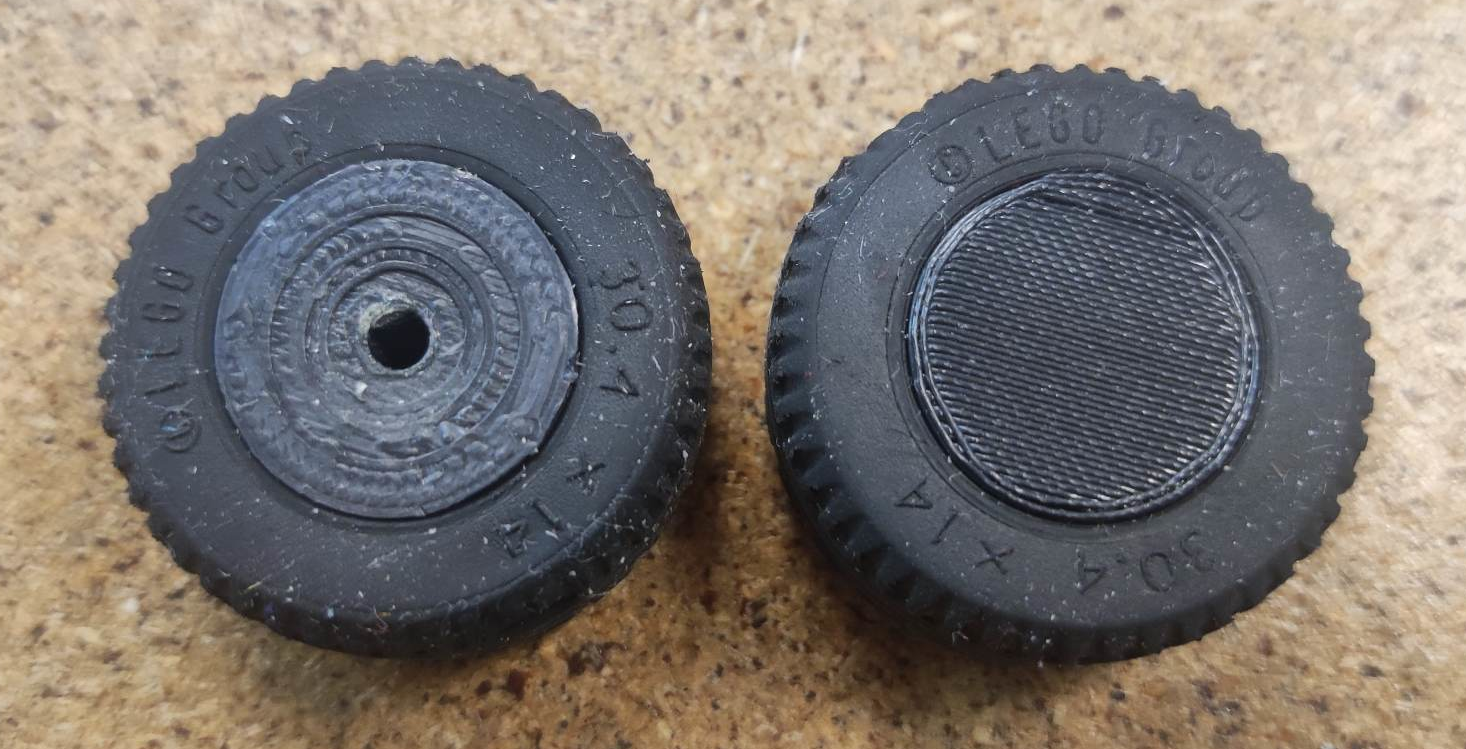
\includegraphics[width=1.4\linewidth]{zdjecia/kola.png}
         \caption{Felgi i opony}\label{Fig:Data1}
       \end{minipage}\hspace{45mm}
       \begin{minipage}{0.3\textwidth}
         \centering
         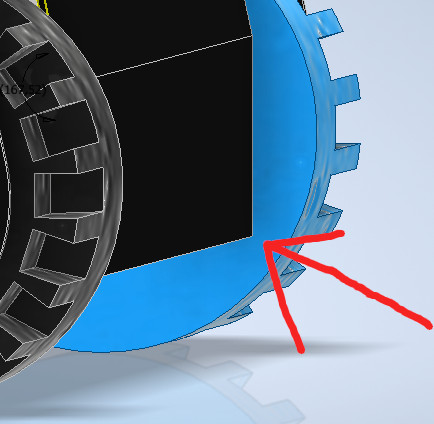
\includegraphics[width=1.1\linewidth]{photo/Kola.jpg}
         \caption{Zbliżenie na koła}\label{Fig:Data2}
       \end{minipage}
        \end{figure}
        
    \subsection{Dociążenie}
        W ostatecznej wersji robota konieczne było użycie ołowianych obciążników w celu dociążenia robota ponieważ bez tego ważył tylko połowe maksymalnej masy. Sprawiło by to że robot nie miał by szans z innymi robotami na zawodach. Przy jego dociążaniu ważne było to aby dobrze rozmieścić mase. Zbyt duża masa z przodu powodowała ślizganie kół. Zbyt duża masa z tyłu podnoszenie się przodu przy gwałtownym cofaniu.
    
    \subsection{Pierwszy prototyp}
        
            
    \begin{figure}[!htb]
       \begin{minipage}{0.3\textwidth}
         \centering
         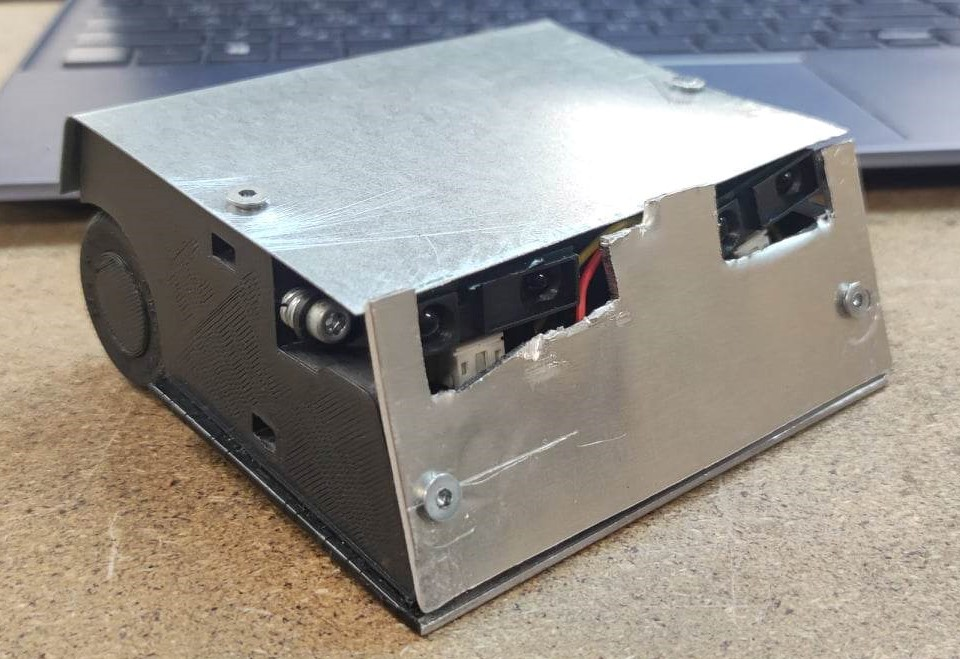
\includegraphics[width=1.55\linewidth]{photo/Pierwszy_przod.jpg}
         \caption{Widok z przodu}\label{Fig:Data1}
       \end{minipage}\hspace{30mm}
       \begin{minipage}{0.3\textwidth}
         \centering
         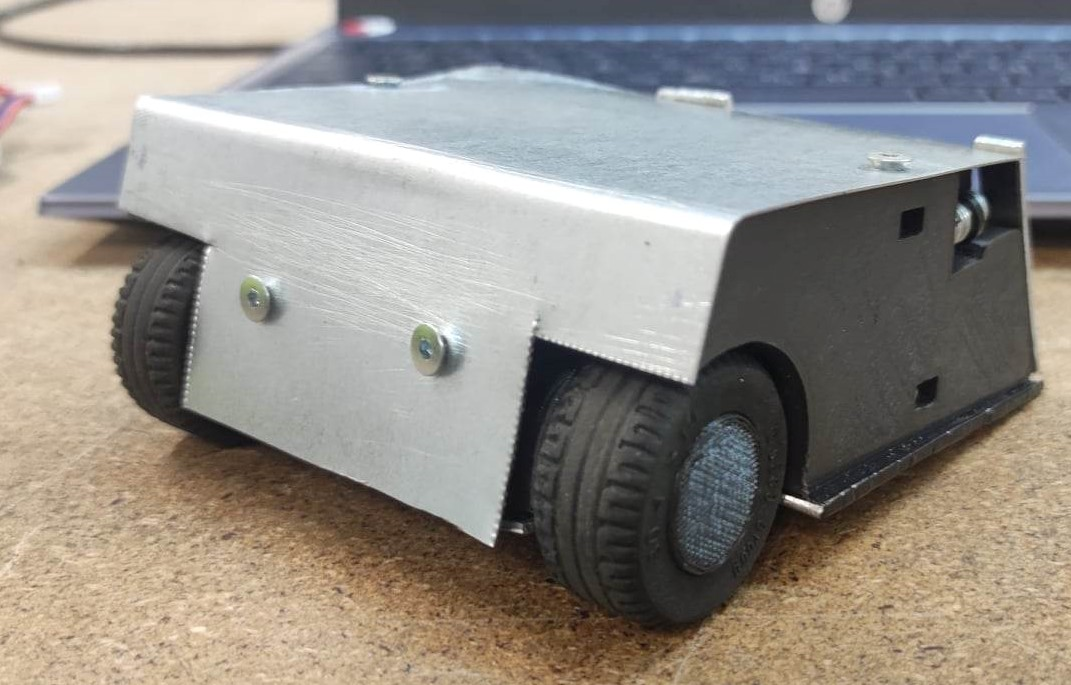
\includegraphics[width=1.65\linewidth]{photo/Pierwszy_tyl.jpg}
         \caption{Widok z tyłu}\label{Fig:Data2}
       \end{minipage}
        \end{figure}
    
    \newpage
    
\section{Program}
    Program robota został napisany w środowisku VSCode przy użyciu wtyczki PlatformIO. 
    Bazą dla całego kodu jest biblioteka "Arduino.h" która zawiera wszystkie podstawowe funkcje. 
    \subsection{Szkielet Programu}



    \begin{figure}[!htb]
       \begin{minipage}{0.3\textwidth}
         
         Szkielet programu oparty jest o następujące bloki:
    
    
        \centering
        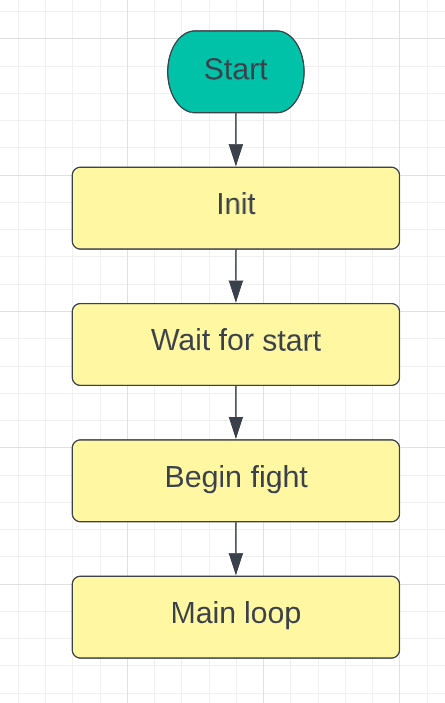
\includegraphics[width=40mm]{Code/glowny.png}
        
       \end{minipage} \hspace{5mm}
       \begin{minipage}{0.7\textwidth}
         
          \textbf{Init} - Zawiera definicje używanych funkcji, ustawienia pinów oraz wszystkie podstawowe instrukcje które są wykonywane po włączeniu zasilania, (np. zapalenie diody informującej o włączeniu zasilania czy ustawieniu wachlarzy w góre).
    \newline
    \textbf{Wait For Start} - Pętla "while" wykonująca się do czasu otrzymania sygnału ze startera. W trakcie trwania pętli dodatkowo za pomocą przycisku można ustalić kierunek, w którym robot skręci po starcie.
    \newline
    \textbf{Begin Fight} - Przygotowanie do walki, wykonywany jest obrót (w lewo lub w prawo, zależnie od wyboru), opuszczanie wachlarzy w dół oraz zaświecenie diody informującej o starcie robota(taka dioda pozwala uniknąć nieporozumień w trakcie zawodów, np. nie odebrania sygnału z pilota). 
    \newline
    \textbf{Main Loop} - główna pętla programu.
    
       \end{minipage}
        \end{figure}




    
    
    
    
   
    \subsection{Główna pętla programu - algorytm walki}
    Algorytm walki robota opiera się głównie o odczyty z czujników odległości, na ich podstawie wykonywane są poszczególne akcje.
    \newline

    
    \begin{figure}[!htb]
       \begin{minipage}{0.3\textwidth}
         
         
    
    
        \centering
        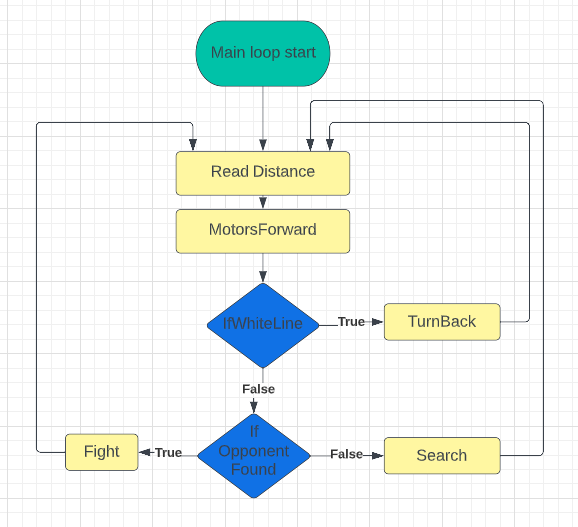
\includegraphics[width=90mm]{Code/MainLoop.png}
        
       \end{minipage} \hspace{42mm}
       \begin{minipage}{0.47\textwidth}
         
    \textbf{ReadDistance} - Odczytanie wartości z czujników odległości oraz zapamiętanie ostatniej pozycji w której został wykryty przeciwnik.
    \newline
    \newline
    \textbf{MotorsForward} - Ustawienie kierunku obrotu silnikami do przodu.
    \newline
    \newline
    \textbf{IfWhiteLine} - Sprawdzenie czy wystąpiła biała linia na podstawie odczytu z czujników podłoża. Jeśli  biała linia wystąpi, robot przerywa jazde do przodu i zawraca w strone zależną od tego po której stronie czujnik podłoża wykrył białą linie. Jest to zabezpieczenie przed wypadnięciem z ringu.
    \newline
    \newline
    \textbf{IfOpponnentFound} - Sprawdza czy w danym odczycie przeciwnik został wykryty.
    


        \end{minipage}
        \end{figure}

    
  \newpage
    
    \subsection{Fight}
    Funkcja "Fight" uruchamiana jest w momencie gdy robot wykrył przeciwnika.

     \begin{figure}[!htb]
       \begin{minipage}{0.3\textwidth}

        \centering
        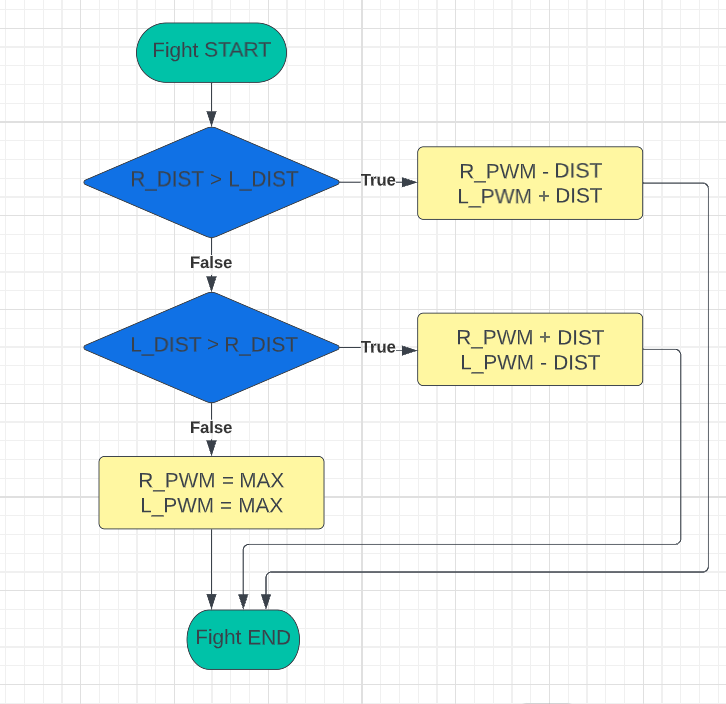
\includegraphics[width=85mm]{Code/fight.png}
        
       \end{minipage} \hspace{37mm}
       \begin{minipage}{0.5\textwidth}
         
        W trakcie jej trwania wykonywane są operacje zmiany szybkości obrotu kół, co pozwala na możliwie najszybsze zepchanie przeciwnika z ringu. W zależności od tego po której stronie czujniki odległości wykryły przeciwnika oraz w jakiej odległości, dobiera odpowiednie wartości PWM. W konsekwencji robot wykonuje skręty o takich kątach które pozwalają na najszybszy kontakt z przeciwnikiem. 
    \newline\newline
    Prościej mówiąc gdy przeciwnik jest blisko, robot wykonuje skręt po krótkim łuku, gdy jest daleko, łuk skrętu jest długi.
    
    Gdy przeciwnik jest odpowiednio blisko, predkości obrotu obydwu kół ustawiane są na maksymalną wartość.
        
       \end{minipage}
        \end{figure}
    
    \subsection{Search}
    Funkcja "Search" uruchamiana jest w momencie gdy robot niczego nie wykrył lub przeciwnik uciekł z pola widzenia. 

    \begin{figure}[!htb]
       \begin{minipage}{0.3\textwidth}

        \centering
        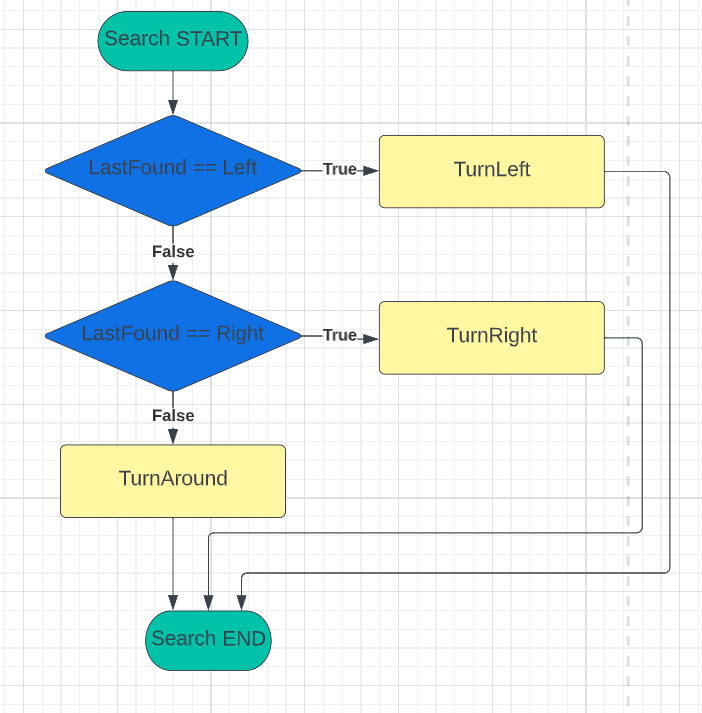
\includegraphics[width=85mm]{Code/search.png}
        
       \end{minipage} \hspace{37mm}
       \begin{minipage}{0.5\textwidth}

         Na podstawie zapamiętanej ostatniej pozycji przeciwnika robot "próbuje" przewidzieć jego obecną pozycje i wykonuje skręt w odpowiednią strone. W momencie, gdy nie dysponuje ostatnią pozycją, stara się znaleźć przeciwnika poprzez obrót dookoła. 
      
       \end{minipage}
        \end{figure}

    
    \subsection{Skręty, obroty i zawroty}
    Dodatkowo należy wspomnieć, że wszystkie funkcje występujące w programie typu: TurnLeft,TurnRight, TurnBack, TurnAround na bieżąco sprawdzają odczyty z czujników odległości i w razie wykrycia przeciwnika przerywają operacje skrętu.
   \newpage
\section{Aktualizacje robota}
    Po stworzeniu wstępnej wersji robota okazało się że niektóre aspekty można znacznie usprawnić.
    \subsection{Nowe koła}
    Bardzo dużym problemem był brak odpowiedniej przyczepności do podłoża, opony z LEGO nie były w stanie tego zapewnić. W wyniku tego robot nie miał szans przy bezpośrednich starciach na przepychanie się. W tym przypadku pomogła zmiana kół na opony odlewane z silikonu. Do testów koła zostały pożyczone z robota "XYZ" autorstwa Tomasza Kozłowskiego.
    
    \begin{figure}[ht!]
        \centering
        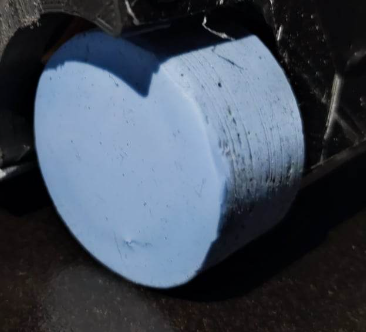
\includegraphics[width=45mm]{zdjecia/Opony.png}
        \caption{Nowe opony \label{overflow}}
        \end{figure}
    
    \subsection{"Technologia wachlarzy" - płachta na byka}
    Dodatkowe techniki usprawniające taktykę walki zawsze sprawiają że robot ma większą szanse na wygraną. Na zawodach w Bukareszcie okazało się że roboty które były na szczycie posiadały wbudowane, opuszczane po starcie "wachlarze". Po zainspirowaniu się najlepszymi zawodnikami wachlarze zostały zaimplementowane również w Stefanie. 

    \begin{figure}[!htb]
       \begin{minipage}{0.3\textwidth}
         \centering
         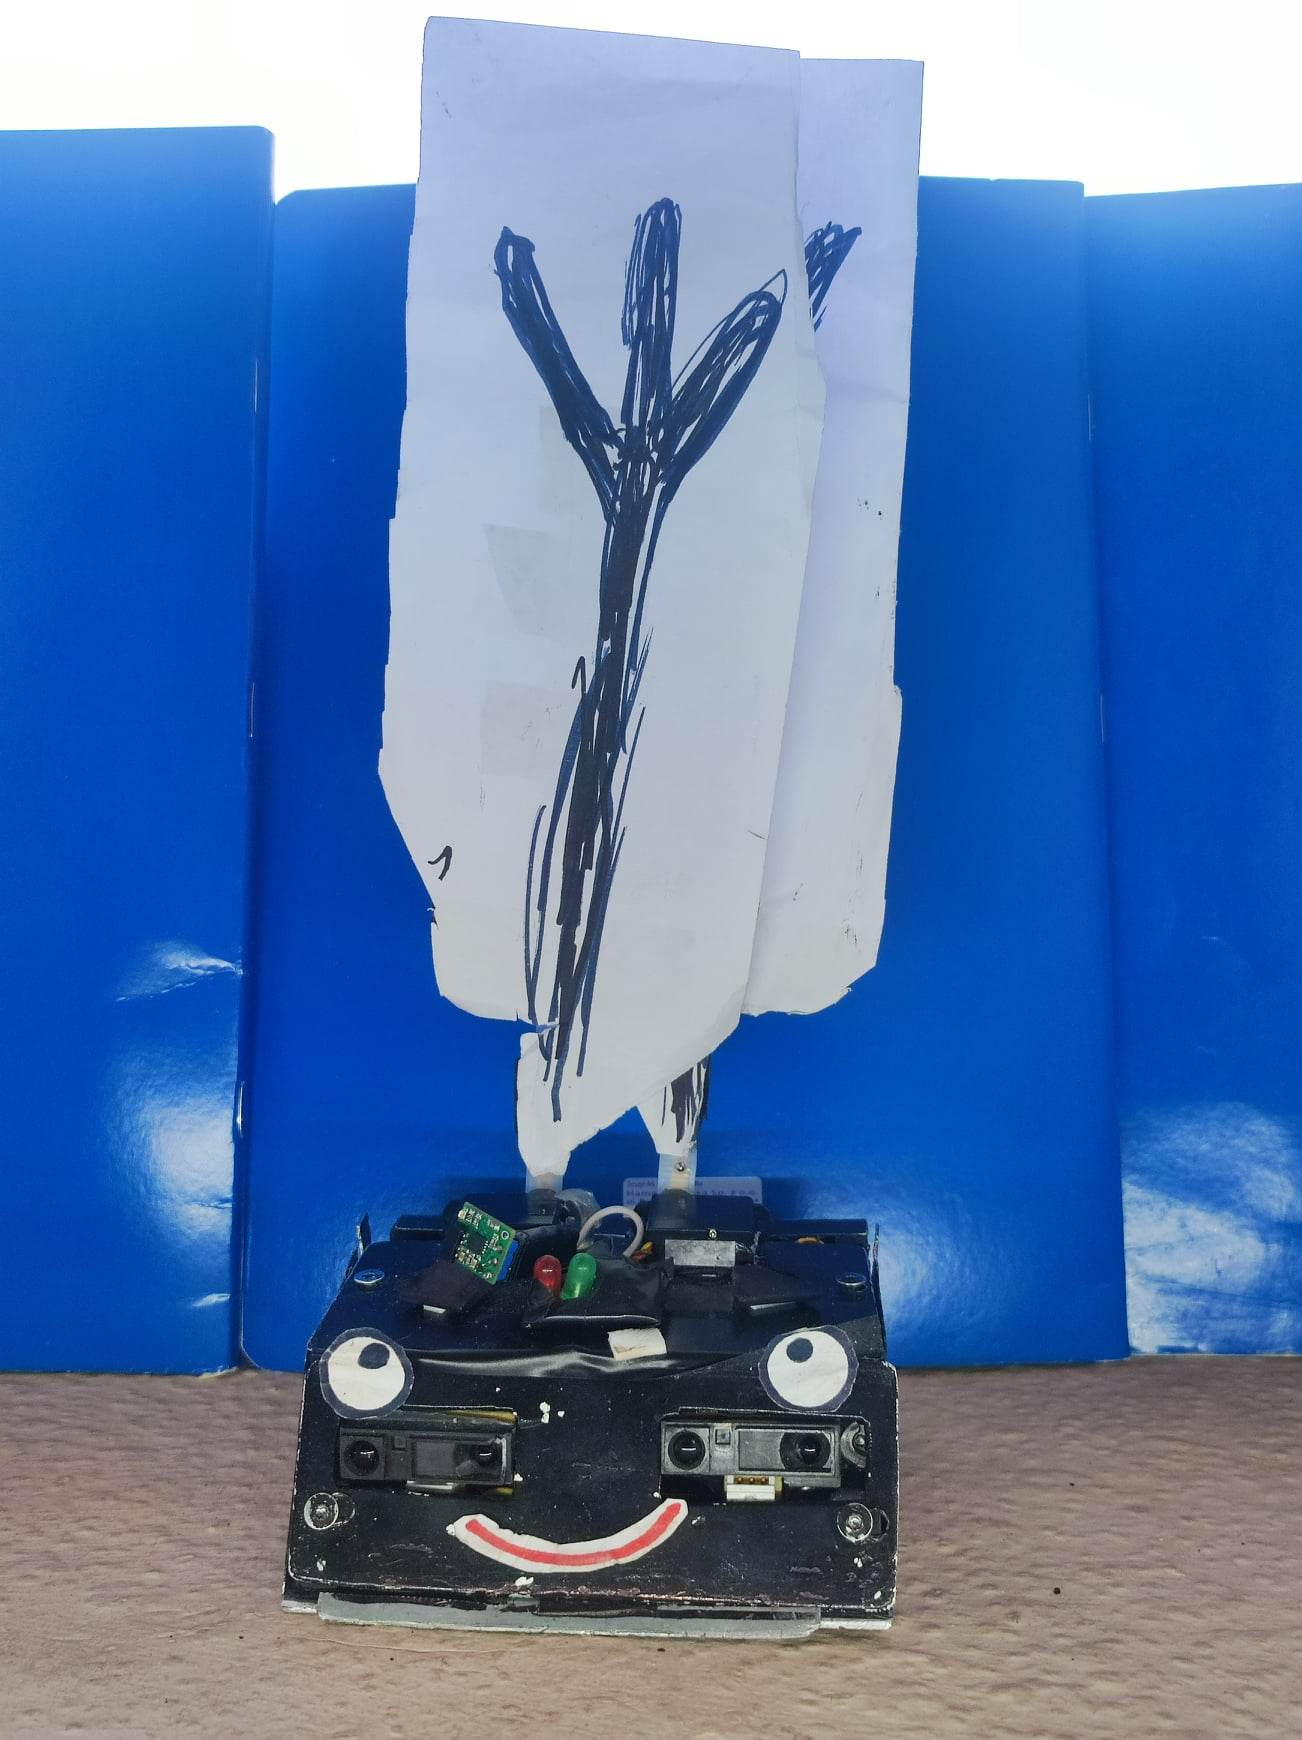
\includegraphics[width=1\linewidth]{zdjecia/zlo.jpg}
         \caption{Pozycja startowa}\label{Fig:Data1}
       \end{minipage}\hspace{0mm}
       \begin{minipage}{0.3\textwidth}
         \centering
         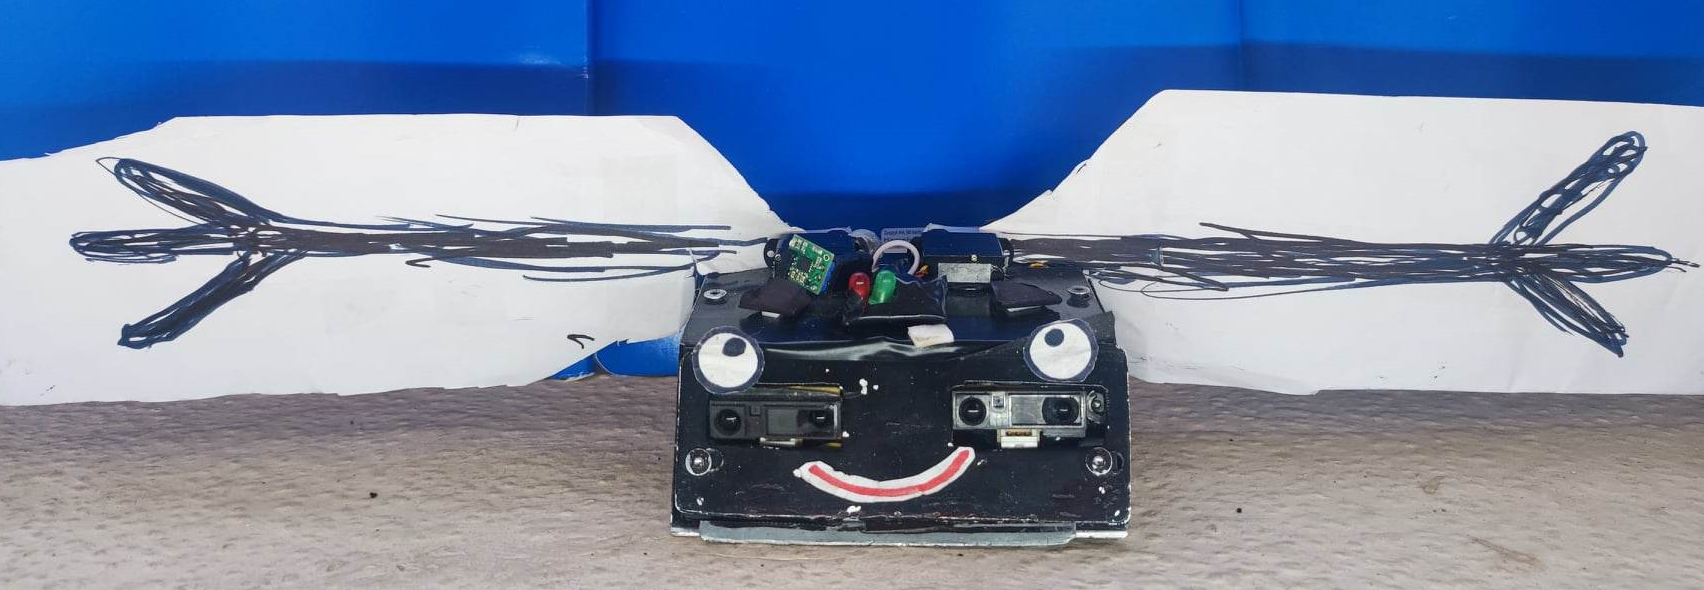
\includegraphics[width=2.4\linewidth]{zdjecia/rozl.png}
         \caption{Pozycja walki}\label{Fig:Data2}
       \end{minipage}
        \end{figure}
    
    Wachlarze w pozycji startowej muszą mieścić się w obrysie robota aby spełniać regulamin. Dopuszcza on zwiększenie rozmiarów robota po starcie, co tutaj bardzo dobrze jest wykorzystywane.
    \newline
    Opuszczane wachlarze sprawiają że nasz robot staje się znacznie trudniejszy do wykrycia ponieważ przeciwnik, który niekoniecznie jest na to przygotowany "myśli" że, w miejscu w którym coś wykrył znajduje się nasz robot. Przeciwnik stara się wtedy z najwyższą prędkością wypchać poza ring naszego robota. Sprawia to że, robot przeciwnika "prześlizguje się" przez wachlarz i sam wypada poza ring. W ostateczności bardzo przeszkadza mu to w wykryciu naszego robota.
    \newline Do opuszczania wachlarzy zostały wykorzystane dwa mikro-serwa.
    
    \subsection{Dodatkowe czujniki odległości}
    Jako kolejne ulepszenie robota planowane są dodatkowe czujniki odległości. Umieszczone obecnie dwa czujniki odległości z przodu robota są nie do końca wystarczające. Robot widzi tylko to co ma przed sobą. Umieszczenie dodatkowych czujników z boku, znacznie poprawiło by zdolność do wykrywania przeciwnika, czym samym do wygrywania walk.
    \subsection{Nowa płytka z elektroniką}
    Jako kolejne ulepszenie chciałbym wykonać projekt płytki PCB, aby elektronika robota była bardziej niezawodna.
    
    
    \section{Wady konstrukcyjne}
    \begin{itemize}
  \item Bateria zastosowana w robocie ma niepotrzebnie tak dużą objętość. Można zastosować mniejszą co sprawiło by że robot mógłby być niższy.
  
  \item  Niezaprzeczalnie jedną z największych wad jest metoda wykonania płytki z elektroniką. Użyty sposób wykonania płytki ma znacznie więcej wad niż zalet oraz nie jest on zbytnio profesjonalny i wytrzymały.Połączenia kabli często ulegały awarii, co znacznie przeszkadzało w pracy przy projekcie.
  
  \item Brak noża dzięki któremu łatwiej jest podważyć przeciwnika.
  
  \item Czujniki odległości umieszczone są za wysoko co sprawia że czasami przeciwnik może zostać niezauważony przez swoją wysokość. 
  
  \item Program robota wymaga sporej optymalizacji ponieważ działa powoli i często robot nie reaguje odpowiednio szybko na wykrycie przeciwnika. Bywają też momenty że przeciwnik w ogóle nie zostanie wykryty.

\end{itemize}
\newpage
\section{Zawody}
    \subsection{RoboChallange Bukareszt 5-6.11.2022}
    Zawody w Bukareszcie były pierwszymi zawodami na jakich Stefan wystartował. Poradził on sobie niespodziewanie dobrze. Wygrał on jedną walkę w grupie, co wystarczyło na przejście do kolejnego etapu - finałów. Dzięki tym zawodom można było przekonać się co w robocie wymaga poprawy i ulepszeń. 
    
    \begin{figure}[ht!]
        \centering
        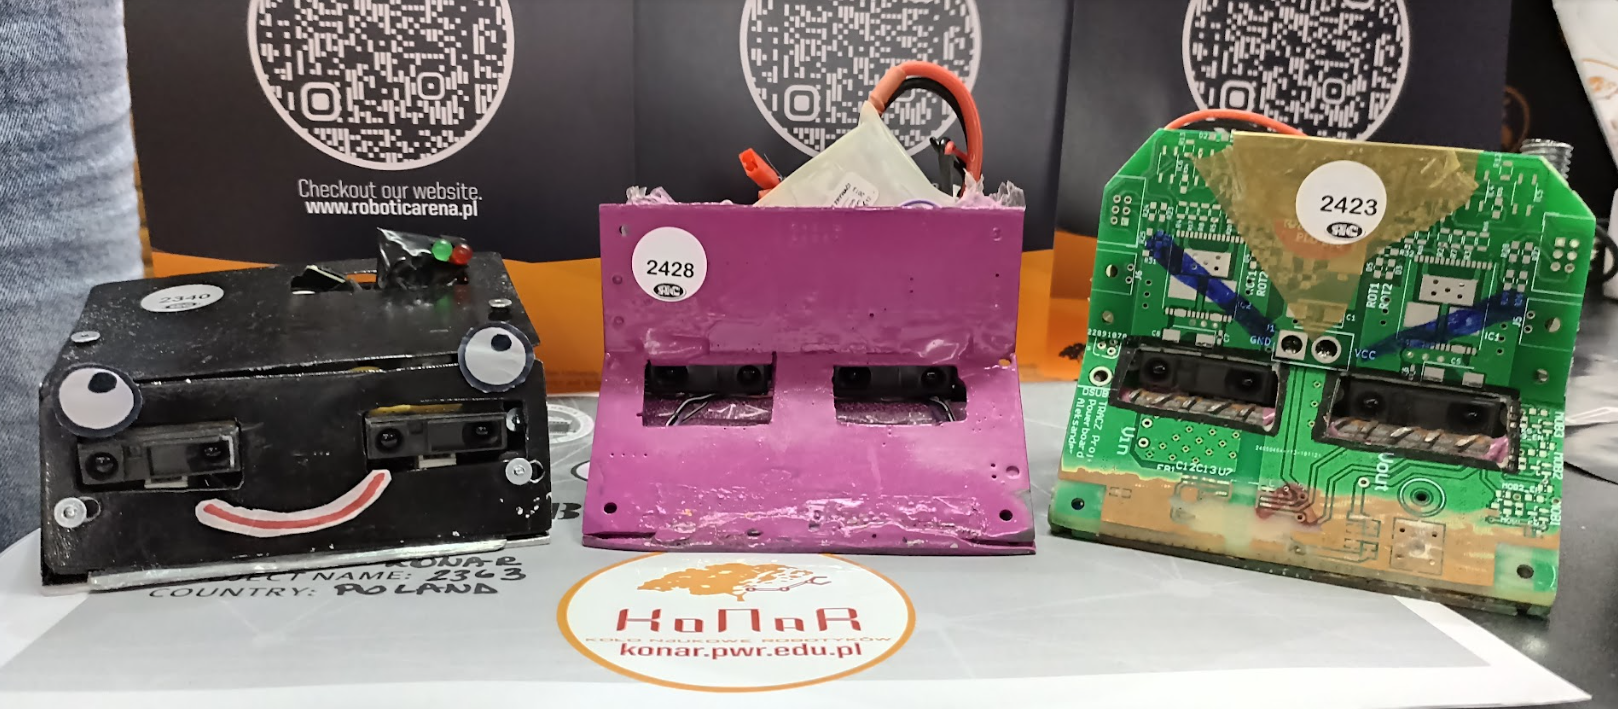
\includegraphics[width=150mm]{zdjecia/StefanZEkipa.png}
        \caption{Stefan z Paskudą i MiniRikishi w Bukareszcie. \label{overflow}}
        \end{figure}
    
    \subsection{Robo ~ Motion Rzeszów 26.11.2022}
    Były to pierwsze zawody Stefana na których był juz wyposażony w nowe koła i wachlarze. Te dwa ulepszenia okazały się znaczące. Po pięknych, dwóch wygranych walkach w grupie, wyszedł z niej na drugim miejscu- przegrywając jedynie z robotem "Er-sześć". Pokonując kolejnych przeciwników ostatecznie zajął 3 miejsce!

    \begin{figure}[!htb]
       \begin{minipage}{0.3\textwidth}
         \centering
         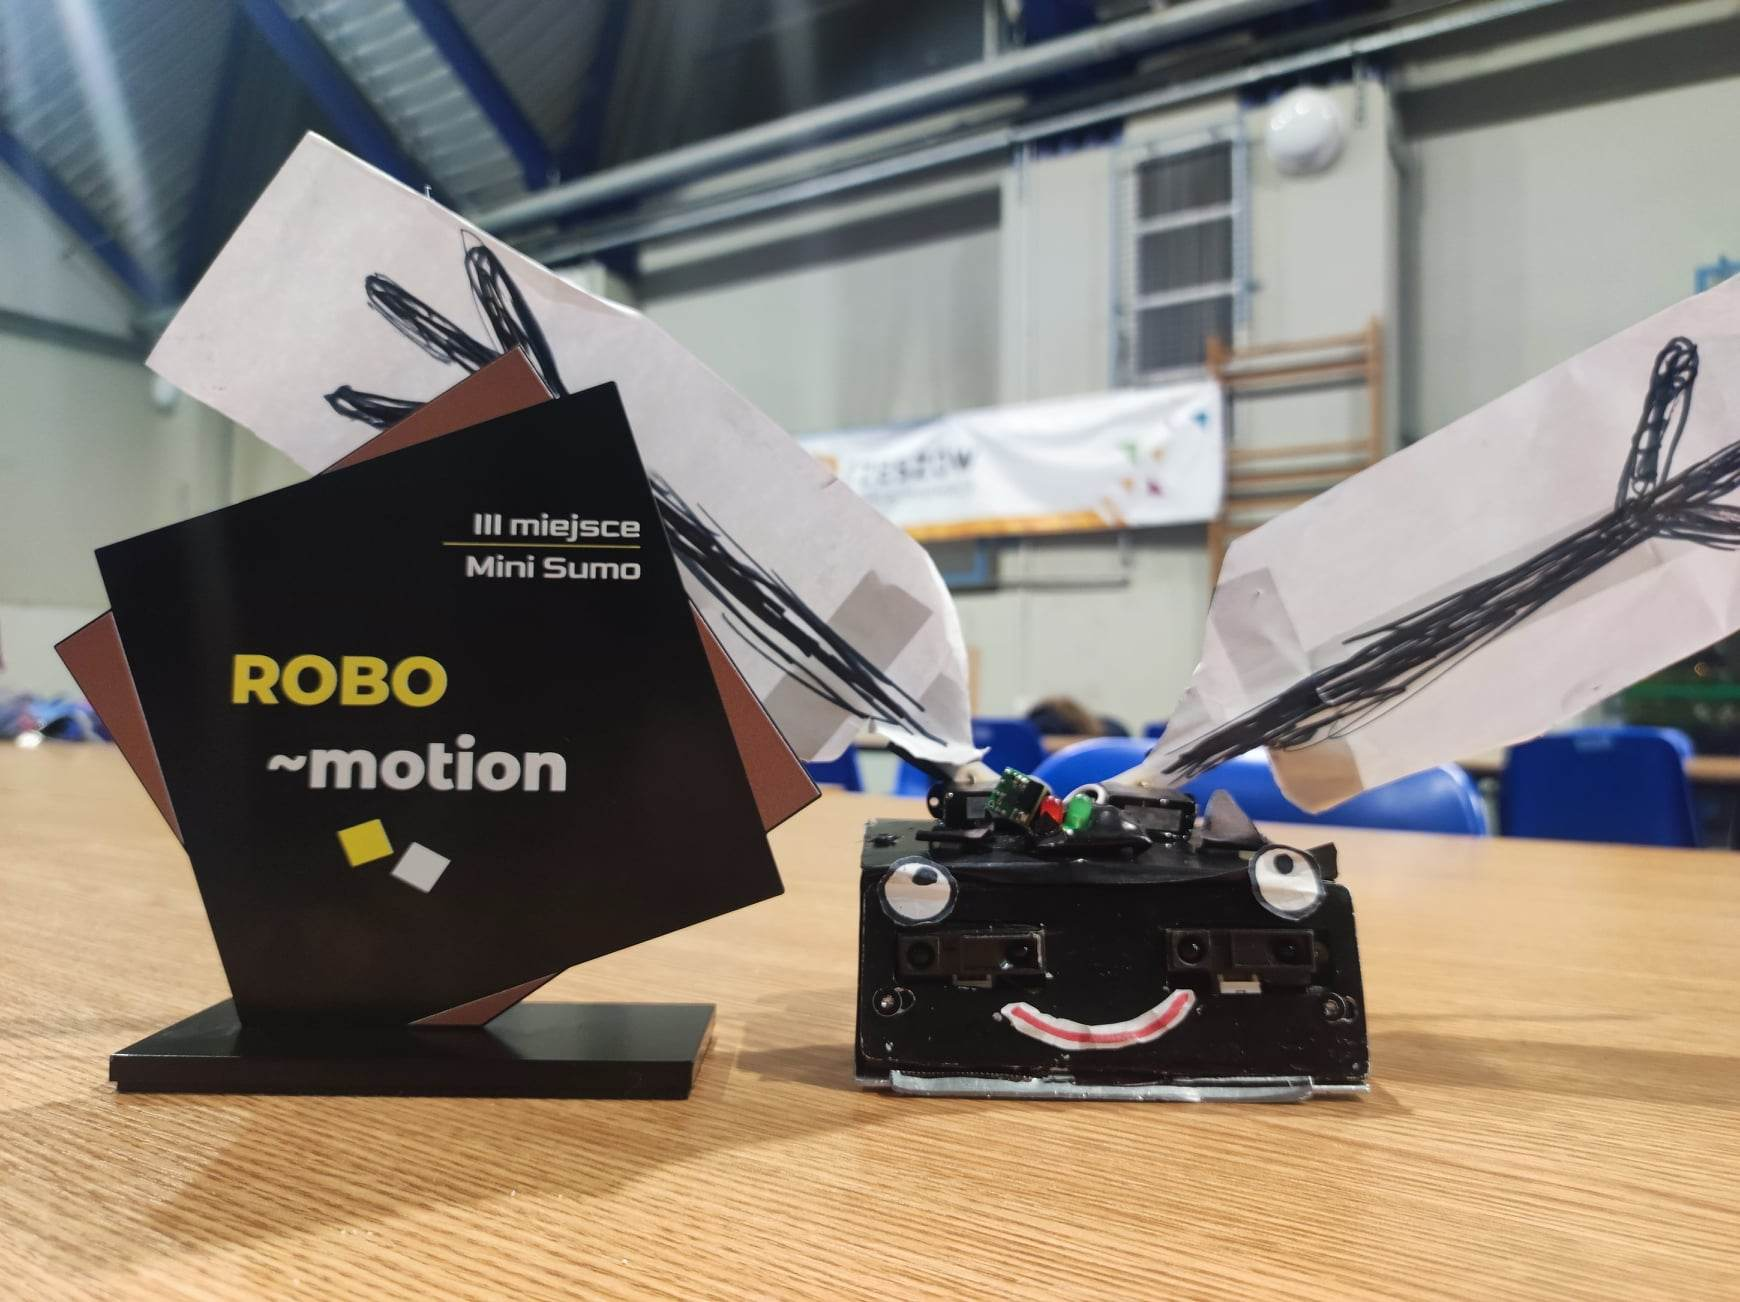
\includegraphics[width=1.55\linewidth]{zdjecia/PoZawodach.jpg}
         \caption{Stefan po zawodach w Rzeszowie}\label{Fig:Data1}
       \end{minipage}\hspace{30mm}
       \begin{minipage}{0.3\textwidth}
         \centering
         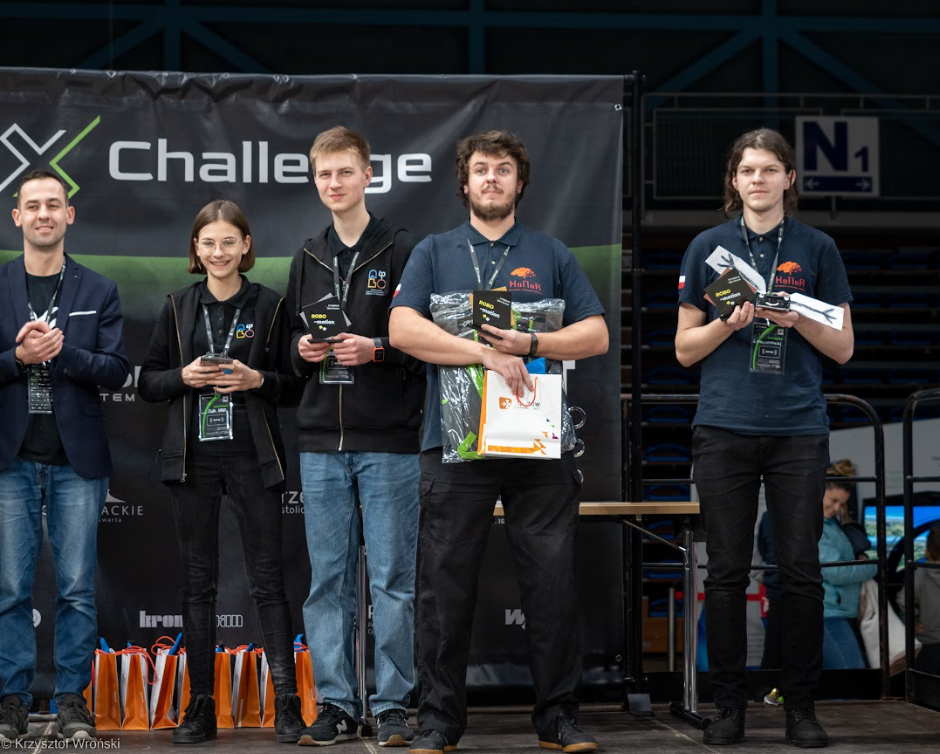
\includegraphics[width=1.65\linewidth]{zdjecia/podium.png}
         \caption{Podium w Rzeszowie}\label{Fig:Data2}
       \end{minipage}
        \end{figure}
    
\bibliographystyle{alpha}
\newpage
\bibliography{}

\begin{itemize}
  \item Eryk Możdzeń - Robot mobilny klasy minisumo„Sneak100”: \url{https://github.com/Eryk-Mozdzen/minisumo-sneak100}
  \item SumoStartModule: \url{https://p1r.se/startmodule/} , \url{https://github.com/p1rse/robot-sumo-start-module}

\end{itemize}




\end{document}


Wiecej informacji na temat startera można znaleźć na \href{https://p1r.se/startmodule/}{stronie} oraz \href{https://github.com/p1rse/robot-sumo-start-module}{GitHubie} twórcy.